% -- Dokumentenbeginn --%
\documentclass[12pt, a4paper]{scrartcl}

% Standard
\usepackage[utf8]{inputenc}
\usepackage[german]{babel}
\usepackage{amsmath}
\usepackage{amsfonts}
\usepackage{amssymb}
\usepackage{graphicx}

% Schriftverbesserung
\usepackage{microtype}
\usepackage{pifont}
\usepackage{xspace}
\usepackage{setspace}

% Code Input
\usepackage{listings}

% Änderung des Abstands von \maketitle
\usepackage{titling}
\setlength{\droptitle}{-2cm}
\parindent0pt

% cite und Co.
\usepackage[plain,german]{fancyref}
\usepackage{hyperref}
\usepackage{float}
\usepackage{lmodern}
\renewcommand*\familydefault{\sfdefault}
\usepackage{setspace}

% eigene commands
\newcommand{\cmark}{\ding{51}}
\newcommand{\xmark}{\ding{55}}

% Kopf
\author{Christopher Sauer}
\title{\textbf{Dokumentation -- Github und Parsor}}
\date{\today}

\begin{document}

\onehalfspacing

\maketitle
\tableofcontents

\vspace{4em}

\listoffigures

\clearpage
\section{Einführung}

Um den Quellcode für Parsor besser zu verwalten, wurde dieser komplett auf die Opensource-Plattform Github \cite{github} hochgeladen. Dies bring folgende Vorteile:

\begin{itemize}
	\item Einfache Einsicht in den Code
	\item Versionsvergleiche
	\item Zusammenarbeit am eigentlichen Code
	\item Verwaltung von Fehlermeldungen und generellen Problemen
	\item Anregungen und Wünsche für neue Funktionen
\end{itemize}

Der Quellcode ist unter \url{https://github.com/Balagrio/Parsor} erreichbar. Dieser wird mit dem Versionsverwaltungssystem \texttt{git} \cite{git} verwaltet. Über die Kommandozeile oder verschiedene grafische Oberflächen wie die offizielle Windows Github-App \cite{git_win}, die App für Macintosh \cite{git_mac} oder ein Github Eclipse Plugin \cite{git_eclipse}. Bei allen Anwendungen wird die \texttt{git} Kommandozeilen-Anwendung mitgeliefert und Github setzt darauf jeweils mit einer grafischen Oberfläche auf. Wer nur das reine \texttt{git} verwenden möchte, dem empfehle ich die Kommandozeile oder die grafische Oberfläche \texttt{mysysgit} \cite{mysysgit}, die sich auch über das Windows-Rechtsklickmenu bedienen lässt.

\clearpage
\section{Fehlermeldungen und Co.}

Ein weiterer Vorteil ist, dass nach einer kurzen Registrierung Fehlerberichte und Co unter dem Reiter "'Issues"' in Github geschrieben werden können, dann kann ich mich dran machen diese Fehler auszumerzen oder neue Funktionen zu implementieren. Fragen, Wünsche, Anregungen gerne auf Github stellen. Auf diese Funktion könnt ihr nach erfolgreicher Registrierung auf der Hauptseite \cite{github} zugreifen, siehe \Fref{fig:issues}. \\

\begin{figure}[H]
\centering %
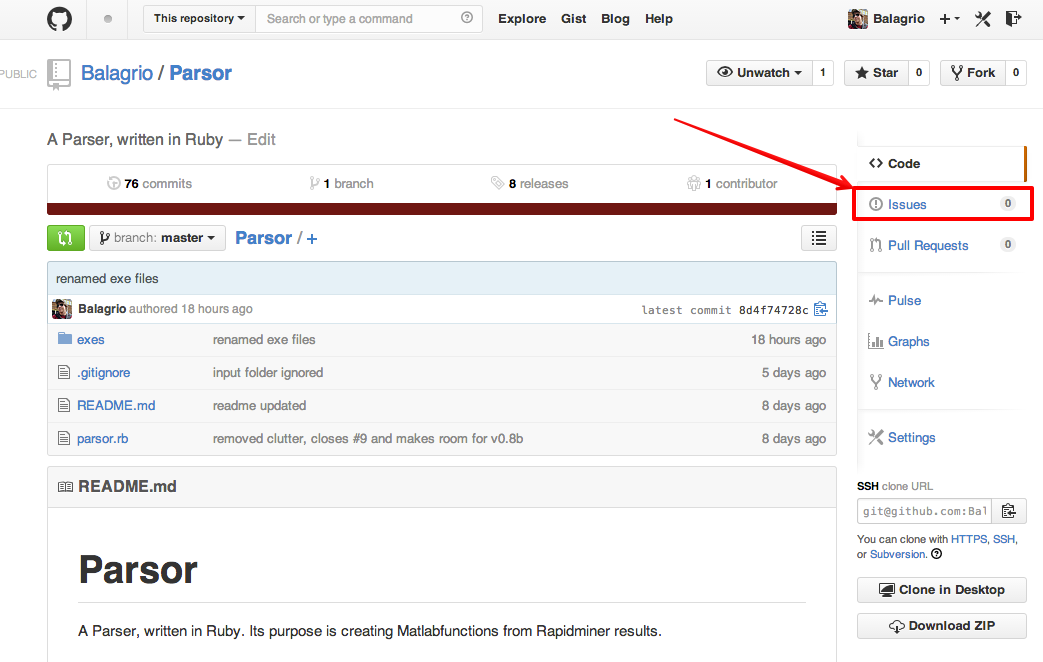
\includegraphics[width=\textwidth]{fig/Issues.png} %
\caption{Github Issues} %
\label{fig:issues} %
\end{figure}

Ich hoffe, dass sich das ganze über Github besser verwalten lässt und Fehler und Co. schneller behoben werden können. 

\clearpage
\section{Aktuelle Parsorversion herunterladen}

Die jeweils aktuelle Parsorversion kann unter \cite{parsor} heruntergeladen werden, siehe \Fref{fig:speichern}. \\

\begin{figure}[H]
\centering %
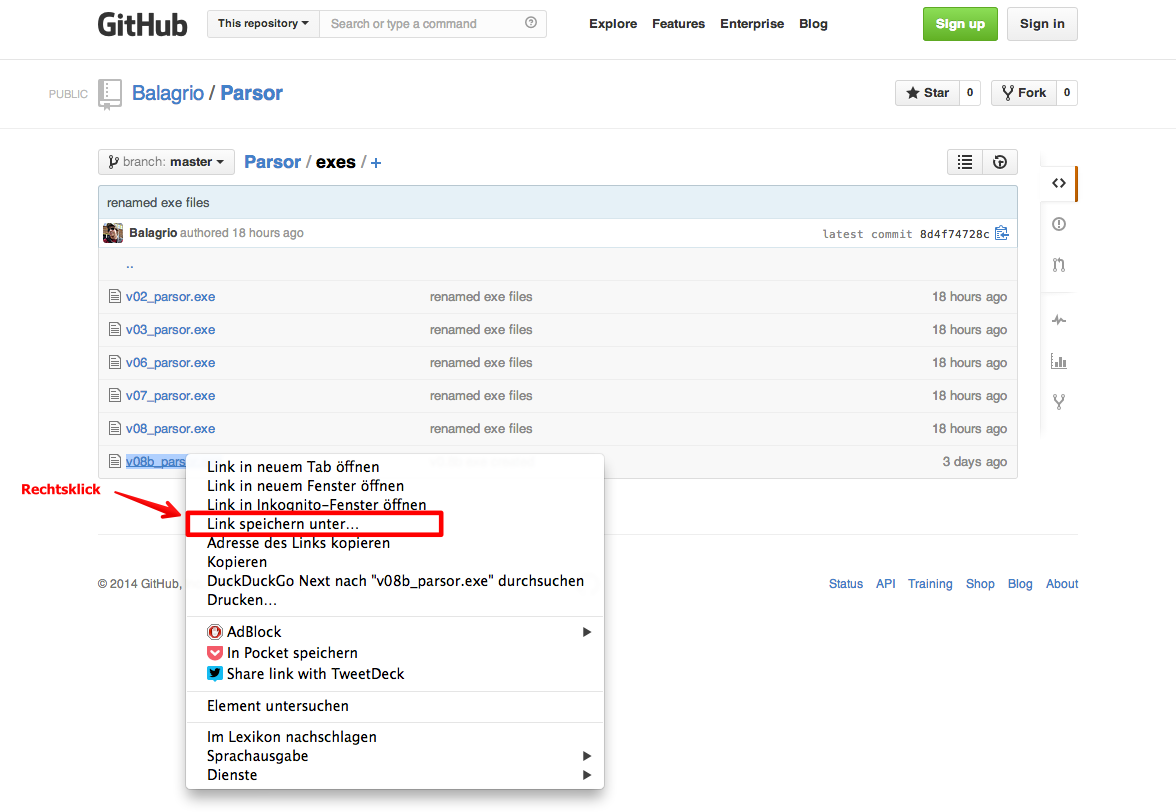
\includegraphics[width=\textwidth]{fig/Speichern.png} %
\caption{Parsor Download} %
\label{fig:speichern} %
\end{figure}

Ich würde mich freuen wenn wir über Github einen Weg finden, Parsor weiter zu verbessern.

\clearpage
\section{Automatischer Aufruf aus Matlab}

Über die \texttt{runparsor.m} Datei lässt sich Parsor auch automatisch aus Matlab aufrufen, dabei können Folgende Optionen gesetzt werden

\begin{enumerate}
	\item Name der Parsor-exe
	\item Verwendetes Verfahren: LR, M5P, M5R, PR
	\item Dateiname der Eingangsdaten
	\item Vorhersage Label bei M5P, M5R 
	\item Erster Buchstabe der Variable
	\item Funktionsname
\end{enumerate}

Ein Beispielaufruf kann sein: \texttt{runparsor('parsor.exe','LR','lr.txt','','X','testfunc')}.

\clearpage
\renewcommand{\refname}{\section{Links}}
\bibliographystyle{plaindin}
\bibliography{links}

\end{document}